\documentclass{beamer}

\usepackage{array}
\usepackage[english]{babel}
\usepackage[utf8x]{inputenc}
\usepackage{amssymb}
\usepackage{amsmath}
\usepackage{booktabs}
\usepackage{graphicx}
\usepackage{datetime}

\title{Research and Adaptation of Components\\from the Persistent OS Phantom for Genode}
\author{student: Mikhail Voronin\\supervisor: Artem Burmyakov\\consultant: Alexander Tormasov}

\newdateformat{monthYear}{\monthname[\THEMONTH] \THEYEAR}
\date{\monthYear\today}

\begin{document}

\frame{\titlepage}

%%%%%%%%%%%%%%%%%%%%%%%%%%%%%%%%%%%%%%%%%%%%%%%%%%%%%%%%%%%

\begin{frame}{Data Persistence}
    \textbf{Data persistence}: period of time during which data exists and is used

    \bigskip
    \textit{R. Morrison, M. P. Atkinson --- ``Persistent Languages and Architectures'', 1990}

    \bigskip\bigskip
    Today's dominant model --- \textbf{two-level store}:
    \begin{itemize}
        \item Data is either \textit{active} (RAM) or \textit{stored} (disk)
        \item Programmer manually moves data between levels
        \item Consequences: data loss, I/O boilerplate ($\approx$30\% of code)
    \end{itemize}
\end{frame}

%%%%%%%%%%%%%%%%%%%%%%%%%%%%%%%%%%%%%%%%%%%%%%%%%%%%%%%%%%%

\begin{frame}{Orthogonal Persistence}
    Alternative: the \textbf{environment} manages persistence

    \bigskip
    Three principles:
    \begin{enumerate}
        \item \textbf{Independence} --- data persistence does not depend on how it is manipulated
        \item \textbf{Data type orthogonality} --- all types can be persisted
        \item \textbf{Identification} --- type does not affect persistence identity
    \end{enumerate}

    \bigskip
    Benefits: up to 30\% reduction in code size, more efficient use of disk bandwidth and improved reliability failt tolerance.
\end{frame}

%%%%%%%%%%%%%%%%%%%%%%%%%%%%%%%%%%%%%%%%%%%%%%%%%%%%%%%%%%%

\begin{frame}{PhantomOS}
    \textbf{PhantomOS} is a non-Unix like OS implementing orthogonal persistence (D. Zavalishin).

    \bigskip
    \begin{itemize}
        \item Persistent Virtual Machine (PVM): bytecode VM + POSIX layer
        \item Snapshots saved periodically via \textbf{Copy-on-Write}
        \item Only changed pages written to disk (incremental)
        \item Programs paused only briefly during snapshot preparation
    \end{itemize}

    \bigskip
    Currently ported to the \textbf{Genode} OS framework:
    \begin{itemize}
        \item Proven microkernels (NOVA, seL4, Fiasco.OC)
        \item Capability-based security, minimal TCB
    \end{itemize}

    \bigskip
    Current snapshot mechanism: \textbf{Snapper}
\end{frame}

%%%%%%%%%%%%%%%%%%%%%%%%%%%%%%%%%%%%%%%%%%%%%%%%%%%%%%%%%%%

\begin{frame}{Snapper}
    File-system-based generational snapshot storage.

    \bigskip
    Previous approach (``superblock''): snapshots stored as monolithic objects.
    \begin{itemize}
        \item[$+$] Fast
        \item[$-$] No fault tolerance, no storage recovery
    \end{itemize}

    \bigskip
    Snapper 2.0:
    \begin{itemize}
        \item Unchanged pages \textbf{linked}, not copied across generations
        \item ext4 + fsck for crash recovery
        \item Integrity checks (hashes per file)
        \item Configurable redundancy policy
    \end{itemize}
\end{frame}

%%%%%%%%%%%%%%%%%%%%%%%%%%%%%%%%%%%%%%%%%%%%%%%%%%%%%%%%%%%

\begin{frame}{Problem Statement}
    PhantomOS snapshots capture the \textbf{entire machine state}\\
    --- including sensitive data present in memory.

    \bigskip
    Snapshots are stored in \textbf{plaintext}.
    An attacker with physical access can mount and read them directly,
    or fully reproduce the machine state.

    \bigskip
    \begin{itemize}
        \item No prior research on this for PhantomOS
        \item No ready-made solution exists in Genode
    \end{itemize}

    \bigskip
    \textbf{Goal}: implement a mechanism for the secure storage of snapshots.
\end{frame}

%%%%%%%%%%%%%%%%%%%%%%%%%%%%%%%%%%%%%%%%%%%%%%%%%%%%%%%%%%%

\begin{frame}{Use Cases \& Requirements}
    Snapshot must remain \textbf{encrypted} at all times.

    \bigskip
    Requirements:
    \begin{enumerate}
        \item Mandatory authorization
        \item Key stored on an \textbf{external USB drive}
        \item Encryption of snapshots (AES, block-level)
        \item Only encrypted data written to disk
        \item Acceptable performance overhead ($\leq 2\times$)
    \end{enumerate}

    \bigskip
    Requirements 1 \& 2 combined: the USB drive contains the key
    and serves as the authentication factor.
\end{frame}

%%%%%%%%%%%%%%%%%%%%%%%%%%%%%%%%%%%%%%%%%%%%%%%%%%%%%%%%%%%

\begin{frame}{Use Cases: Supported Scenarios}
    \begin{center}
        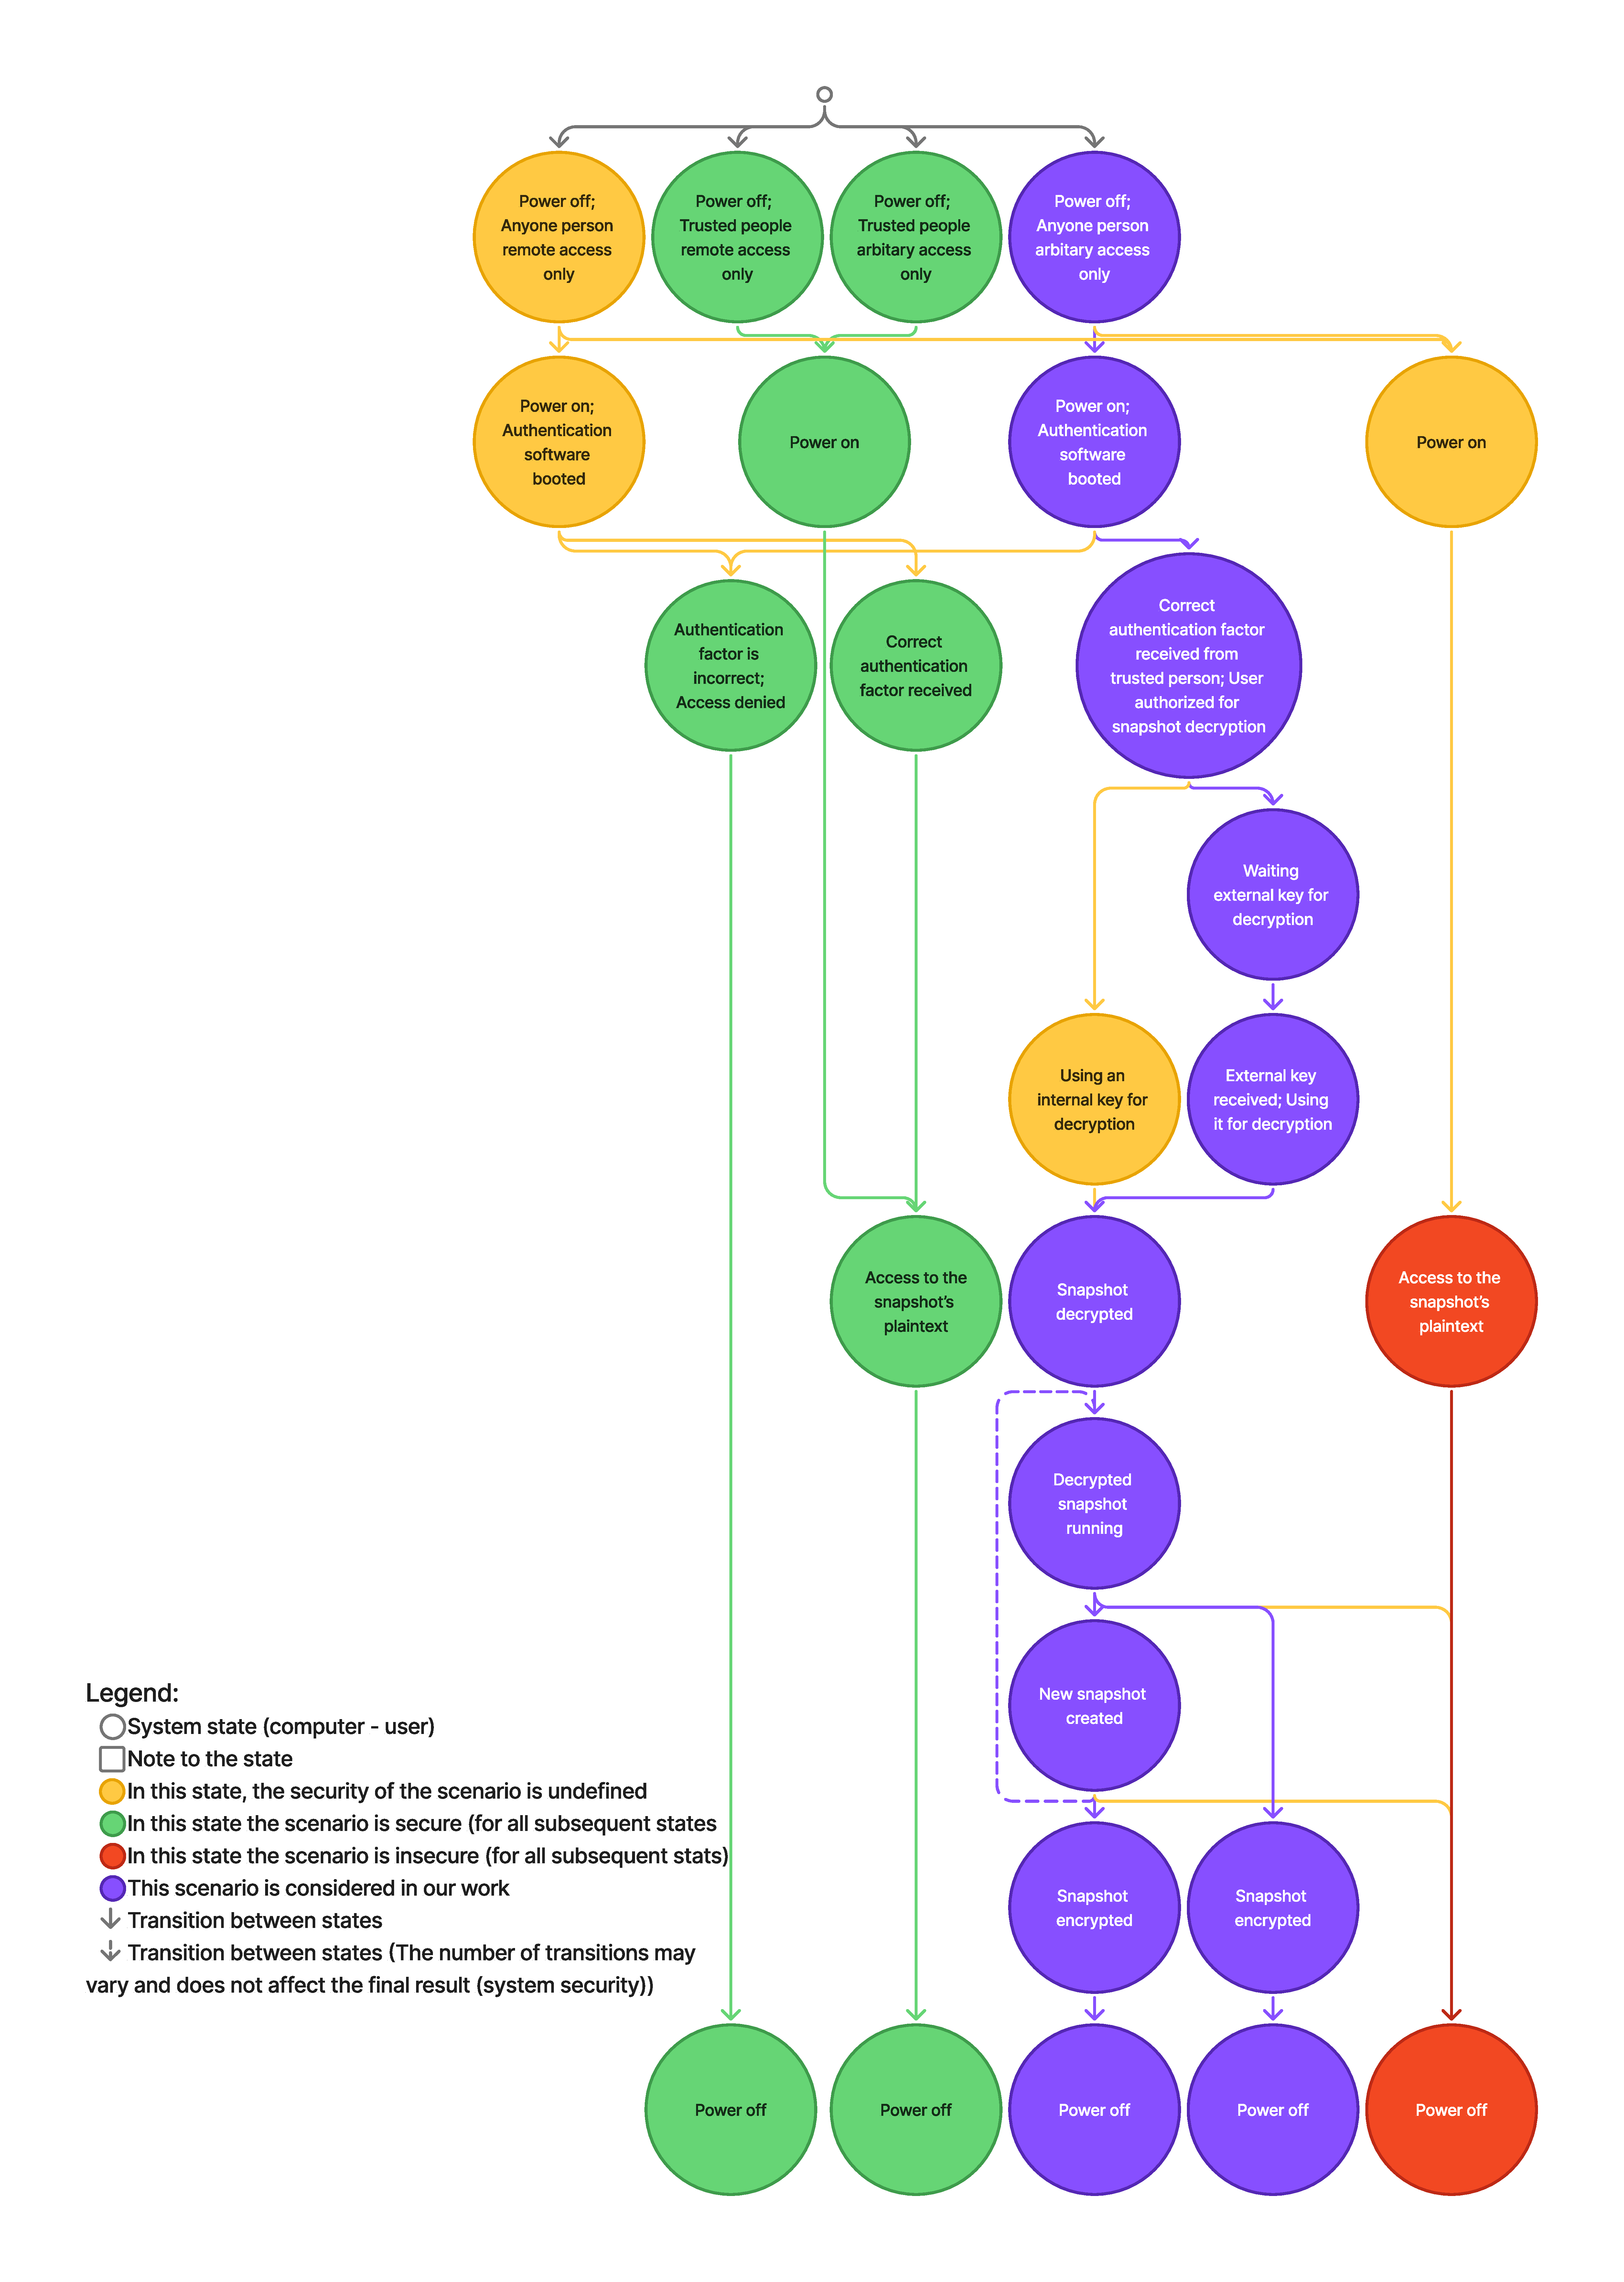
\includegraphics[height=0.85\textheight]{src/use_cases_supported.pdf}
    \end{center}
\end{frame}

%%%%%%%%%%%%%%%%%%%%%%%%%%%%%%%%%%%%%%%%%%%%%%%%%%%%%%%%%%%

\begin{frame}{Implementation: se\_vault}
    There is a \textbf{file\_vault} in Genode based on \textbf{Tresor} library:
    \begin{itemize}
        \item Tresor: AES encryption on 4K blocks, SHA-256 integrity, CoW atomicity
        \item file\_vault: state orchestrator providing a secure FS session
    \end{itemize}

    \bigskip
    Adapted file\_vault $\to$ \textbf{se\_vault}:
    \begin{itemize}
        \item GUI removed --- headless operation
        \item Passphrase replaced by \textbf{USB key file}
        \item rump\_fs/ext2 replaced by \textbf{lwext4/ext4}
        \item Added \textbf{fsck} crash recovery support with fsck
        \item Direct block session (skip image file creation)
        \item All block sizes standardized to 4K
        \item Graceful shutdown sequence added
    \end{itemize}
\end{frame}

%%%%%%%%%%%%%%%%%%%%%%%%%%%%%%%%%%%%%%%%%%%%%%%%%%%%%%%%%%%

\begin{frame}{Related Fixes \& Adaptations}
    \textbf{lwext4} bug fixes:
    \begin{itemize}
        \item \texttt{ftruncate}: pointer cast for correct file size
        \item \texttt{sync} call now propagated to lower VFS layers\\
              (critical --- Tresor updates its state hash on \texttt{sync})
    \end{itemize}

    \bigskip
    \textbf{Shutdown sequence} (isomem / snapper / VFS):
    \begin{itemize}
        \item isomem: power-off button triggers final snapshot
        \item snapper, VFS: client counters trigger graceful shutdown
        \item lwext4 unmounted cleanly; mount flag cleared for fsck
    \end{itemize}

    \bigskip
    \textbf{Optimization}: skipping image file pre-allocation\\
    reduced initialization time from $\approx$20 min to $\approx$1 min.
\end{frame}

%%%%%%%%%%%%%%%%%%%%%%%%%%%%%%%%%%%%%%%%%%%%%%%%%%%%%%%%%%%

\begin{frame}{Testing}
    Environment: QEMU with \texttt{-cpu host} (enables AES/SHA hardware acceleration).\\
    2 GB image for isomem, 5 GB image for se\_vault (4 GB user FS).

    \bigskip
    Functional tests (all passed):
    \begin{itemize}
        \item Normal boot / shutdown / restore cycle
        \item Encrypted image cannot be mounted without key
        \item Key/hash replacement attack --- superblock not detected
        \item Crash recovery via fsck
    \end{itemize}

    \bigskip
    Performance: first snapshot creation and restore, 5 runs each.
\end{frame}

%%%%%%%%%%%%%%%%%%%%%%%%%%%%%%%%%%%%%%%%%%%%%%%%%%%%%%%%%%%

\begin{frame}{Results}
    \begin{center}
    \begin{tabular}{lrrr}
        \toprule
        Operation & Without enc. & With enc. & Overhead \\
        \midrule
        Snapshot creation & 2.10 s & 51.00 s & $\approx 24\times$ \\
        Snapshot restore  & 2.50 s & 27.30 s & $\approx 11\times$ \\
        \bottomrule
    \end{tabular}
    \end{center}

    \bigskip
    Root cause: \textbf{known Tresor library limitation} ---
    not optimized for multithreading.
    Acknowledged by the author; unresolved.
\end{frame}

%%%%%%%%%%%%%%%%%%%%%%%%%%%%%%%%%%%%%%%%%%%%%%%%%%%%%%%%%%%

\begin{frame}{Evaluation}
    \textbf{4 of 5 requirements met.}

    \bigskip
    \begin{tabular}{cl}
        $\checkmark$ & Mandatory authorization (USB key) \\
        $\checkmark$ & Key on external medium \\
        $\checkmark$ & AES block-level encryption \\
        $\checkmark$ & Only encrypted data on disk \\
        $\times$     & Overhead $\leq 2\times$ \textit{(Tresor limitation)} \\
    \end{tabular}

    \bigskip
    Security gain: snapshot cannot be mounted or read without the key.\\
    Integrity: SHA-256 at block level (Tresor) + hash at FS level (Snapper).
\end{frame}

%%%%%%%%%%%%%%%%%%%%%%%%%%%%%%%%%%%%%%%%%%%%%%%%%%%%%%%%%%%

\begin{frame}{Conclusion}
    Adapted \textbf{file\_vault} $\to$ \textbf{se\_vault} for encrypted snapshot storage in PhantomOS on Genode.

    \bigskip
    First security research specifically for PhantomOS.\\
    No analogous component existed prior to se\_vault.

    \bigskip
    Future work:
    \begin{itemize}
        \item Fix Tresor performance (or switch to FS-level encryption via OpenSSL)
        \item Encrypt the isomem block device using se\_vault
        \item Investigate merging Snapper and Tresor snapshot concepts
    \end{itemize}
\end{frame}

%%%%%%%%%%%%%%%%%%%%%%%%%%%%%%%%%%%%%%%%%%%%%%%%%%%%%%%%%%%

\end{document}
